\chapter{Arhitektura i dizajn sustava}

		Na najvišoj razini apstrakcije naš sustav podijeljen je na klijenta i poslužitelja koji komunicira s bazom podataka.
		
		Pomoću web preglednika korisnik se povezuje na web stranicu preko HTTP-a na kojoj interagira s klijentskim dijelom sustava, dakle korisničkim sučeljem. Zahtjevi koje šalje korisnik obrađuje poslužitelj koji po potrebi sprema i preuzima podatke iz baze te vraća korisniku preko klijenta povratnu informaciju.
	
		Arhitektura sustava našeg programskog rješenja dizajnirana je suvremenim pristupom, rabeći Model-View-Controller (MVC) paradigmu koja osigurava smislenu podjelu sustava na manje cjeline prema funkcionalnosti i povezuje backend pisan u C\#-u uz ASP.NET radni okvir, frontend razvijen u htmx-u i JavaScriptu i bazu podataka ostvarenu PostgreSQL-om.


		\begin{itemize}
			\item \textbf{Model:} Mozak sustava, zadužen je za procesuiranje, spremanje i obradu podataka, izvođenje funkcija i općenitog rada sustava. 
			\item \textbf{Controller:} Poput mosta, povezuje sustav s korisničkim unosima. Provodi preliminarnu obradu zahtjeva i prosljeđuje ih modelu i pogledu.
			\item \textbf{View:} Sadrži stvari koje se prikazuju korisniku preko sučelja aplikacije te površinske funkcionalnosti interakcije s korisnikom i promjena prikaza.
		\end{itemize}
		
		\subsection*{Radni tijek}
		
		\begin{itemize}
			\item Korisnik rabi web aplikaciju preko sučelja, šaljući zahtjeve poput unosa teksta u tražilicu.
			\item Kontroler prima zahtjeve, obrađuje ih i prenosi ih modelu.
			\item Model prema potrebi komunicira s bazom podataka, dohvaća potrebne podatke i ispunjava zahtjev.
			\item Kontroler prima procesuirane podatke od modela i prosljeđuje ih pogledu gdje se podaci dinamički predstavljaju korisniku.
		\end{itemize}
				
		\section{Baza podataka}
		
		
		Za potrebe naše aplikacije koristimo relacijsku bazu podataka kako bismo lakše spremili i dohvaćali potrebne podatke. Baza se temelji na relacijama, tj. na tablicama definiranim imenom i atributima.
		
		\subsection{Opis tablica}
		
		Ova tablica sadrži sve potrebne informacije o korisniku, kao što su:
		korisničko ime, lozinku korisnika, korisnikovo ime i prezime, koja je vrsta korisnika, njegov e-mail, broj mobitela, stanje odobrenosti, adresu, grad i državau u kojoj se nalazi. Ona je u
		u One-to-Many vezi s tablicom Knjiga preko svojeg ID-a.
		\begin{longtblr}[
			label=none,
			entry=none
			]{
				width = \textwidth,
				colspec={|X[6,l]|X[6, l]|X[20, l]|}, 
				rowhead = 1,
			} %definicija širine tablice, širine stupaca, poravnanje i broja redaka naslova tablice
			\hline \SetCell[c=3]{c}{\textbf{Korisnik}}	 \\ \hline[3pt]
			\SetCell{LightGreen}ID ponuditelj & INT	&  Jedinstveni identificator korisnika u tablici	\\ \hline
			korisnicko ime	& VARCHAR & korisničko ime izdavača, antikvarijata ili preprodavača  	\\ \hline 
			lozinka & VARCHAR & lozinka korisnika  \\ \hline 
			naziv korisnika & VARCHAR	& ime i prezime korisnika 		\\ \hline 
			vrsta korisnika & VARCHAR	& korisnik može biti izdavač, antikvarijat ili preprodavač 		\\ \hline 
			email & VARCHAR	& e-mail korisnika		\\ \hline 
			broj mobitela & INT	& korisnikov broj mobitela		\\ \hline 
			adresa & VARCHAR	& adresa korisnika 		\\ \hline 
			odobren & BOOLEAN	& govori nam je li korisnik odobren (registriran) u sustavu, tj. može li se ulogirati		\\ \hline 
			drzava & VARCHAR	& država u kojoj se nalazi korisnik 		\\ \hline 
			grad & VARCHAR	& grad u kojem se nalazi korisnik 		\\ \hline 
			
			
		\end{longtblr}
		Ova tablica sadrži sve potrebne informacije o knjigama, kao što su:
		naziv, ime i prezime autora, godina izdanja, naziv i vrstu izdavača, ISBN, broj
		izdanja, opis knjige, jezik na kojem je izdan i dostupnost. Ona je u
		One-to-One vezi s tablicom Korica preko svojeg ID-a, u Many-To-One vezi s tablicom Korisnik preko njezinog ID-a i u One-to-Many vezi s tablicom Ponuda preko svojeg ID-a.
		
		
		\begin{longtblr}[
			label=none,
			entry=none
			]{
				width = \textwidth,
				colspec={|X[6,l]|X[6, l]|X[20, l]|}, 
				rowhead = 1,
			} %definicija širine tablice, širine stupaca, poravnanje i broja redaka naslova tablice
			\hline \SetCell[c=3]{c}{\textbf{Knjiga}}	 \\ \hline[3pt]
			\SetCell{LightGreen}ID naslov & INT	&  Jedinstveni identificator knjige u tablici	\\ \hline
			naziv	& VARCHAR & naziv knjige   	\\ \hline 
			autor & VARCHAR & ime i prezime autora  \\ \hline 
			godina izdavanja & INT	& godina u kojoj je izdana knjiga 		\\ \hline 
			izdavac & VARCHAR	& naziv izdavača knjige 		\\ \hline 
			kategorija izdavaca & VARCHAR	& vrsta izdavača (domaći ili strani)		\\ \hline 
			zanr & VARCHAR	& žanr knjige		\\ \hline 
			ISBN & INT	& međunarodni identificator knjiga 		\\ \hline 
			broj izdanja & INT	& broj trenutnog izdanja knjige	\\ \hline 
			opis & VARCHAR	& kratki opis o radnji knjige		\\ \hline
			jezik & VARCHAR	& jezik na kojem je izdana knjiga 		\\ \hline
			dostupnost & VARCHAR & trenutna dostupnost knjige \\ \hline
			\SetCell{LightBlue} ID ponuditelj	& INT &  Identificator korisnika iz tablice Korisnik 	\\ \hline 
			
			
		\end{longtblr}
		
		
		
		Ova tablica sadrži sve potrebne informacije o dostupnim ponudama, kao što su:
		cijena knjige i broj dostupnih knjiga. Ona je u
		u Many-to-One vezi s tablicom Knjiga preko njezinog ID-a.
		\begin{longtblr}[
			label=none,
			entry=none
			]{
				width = \textwidth,
				colspec={|X[6,l]|X[6, l]|X[20, l]|}, 
				rowhead = 1,
			} %definicija širine tablice, širine stupaca, poravnanje i broja redaka naslova tablice
			\hline \SetCell[c=3]{c}{\textbf{Ponuda}}	 \\ \hline[3pt]
			\SetCell{LightGreen}ID & INT	&  Jedinstveni identificator ponude u tablici	\\ \hline
			cijena	& FLOAT & cijena u eurima po kojoj se knjiga nudi	\\ \hline
			stanje & VARCHAR	& trenutno stanje očuvanosti knjige \\ \hline 
			broj primjeraka	& INT & trenutni broj dostupnih knjiga	\\ \hline 
			\SetCell{LightBlue} ID knjige	& INT &  Identificator knjige iz tablice Knjiga  	\\ \hline 
			
		\end{longtblr}
		Ova tablica sadrži slike korica knjiga. Ona je u 
		One-to-One vezi s tablicom Knjiga ID-a od knjige.
		\begin{longtblr}[
			label=none,
			entry=none
			]{
				width = \textwidth,
				colspec={|X[6,l]|X[6, l]|X[20, l]|}, 
				rowhead = 1,
			} %definicija širine tablice, širine stupaca, poravnanje i broja redaka naslova tablice
			\hline \SetCell[c=3]{c}{\textbf{Korica}}	 \\ \hline[3pt]
			\SetCell{LightGreen}ID & INT	&  Jedinstveni identificator korice u tablici	\\ \hline
			slika	& BLOB & Slika korice (spremljeno u bazi u BLOB formatu)	\\ \hline 
			\SetCell{LightBlue} ID naslov	& INT &  Identificator knjige iz tablice Knjiga  	\\ \hline 
			
		\end{longtblr}
		
		
		
		\subsection{Dijagram baze podataka}
		
		\begin{figure}[hbt!]
			\centering
			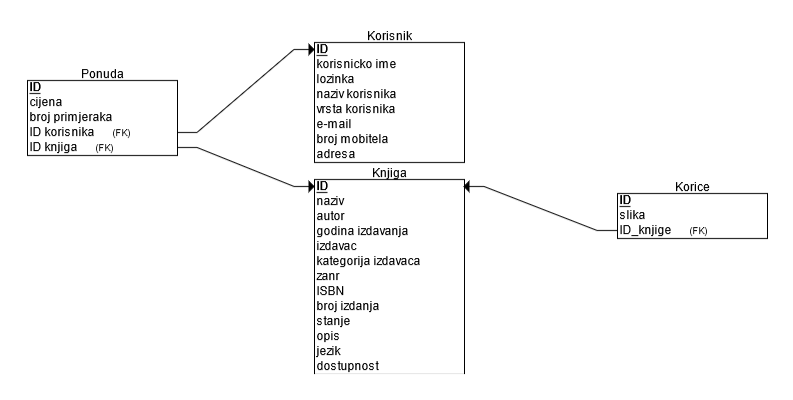
\includegraphics[width = \textwidth]{slike/Relacijska shema}
			\caption{Slika relacijske sheme}
			\label{fig:enter-label}
		\end{figure}
		
		\eject
			
		\section{Dijagram razreda}
		
			\raggedright{Razred Knjiga predstavlja jednu knjigu koja se može pronaći na stranici. Razred Neregistrirani predstavlja korisnika koji može samo pretraživati knjige. Razred registrirani predstavlja korisnika koji sustav koristi za ponudu knjiga. Izdavač, Antikvarijat i Preprodavač su razredi koji predstavljaju različite vrste registriranog korisnika. Svaki registrirani korisnik je jedna od tih tri vrste i zbog toga je razred Registrirani apstraktan. Razred Ponuda predstavlja ponudu jedne knjige. Razred VrstaKnjige predstavlja vrstu svake knjige.}\\
			
			\begin{figure}[h]
				\centering
				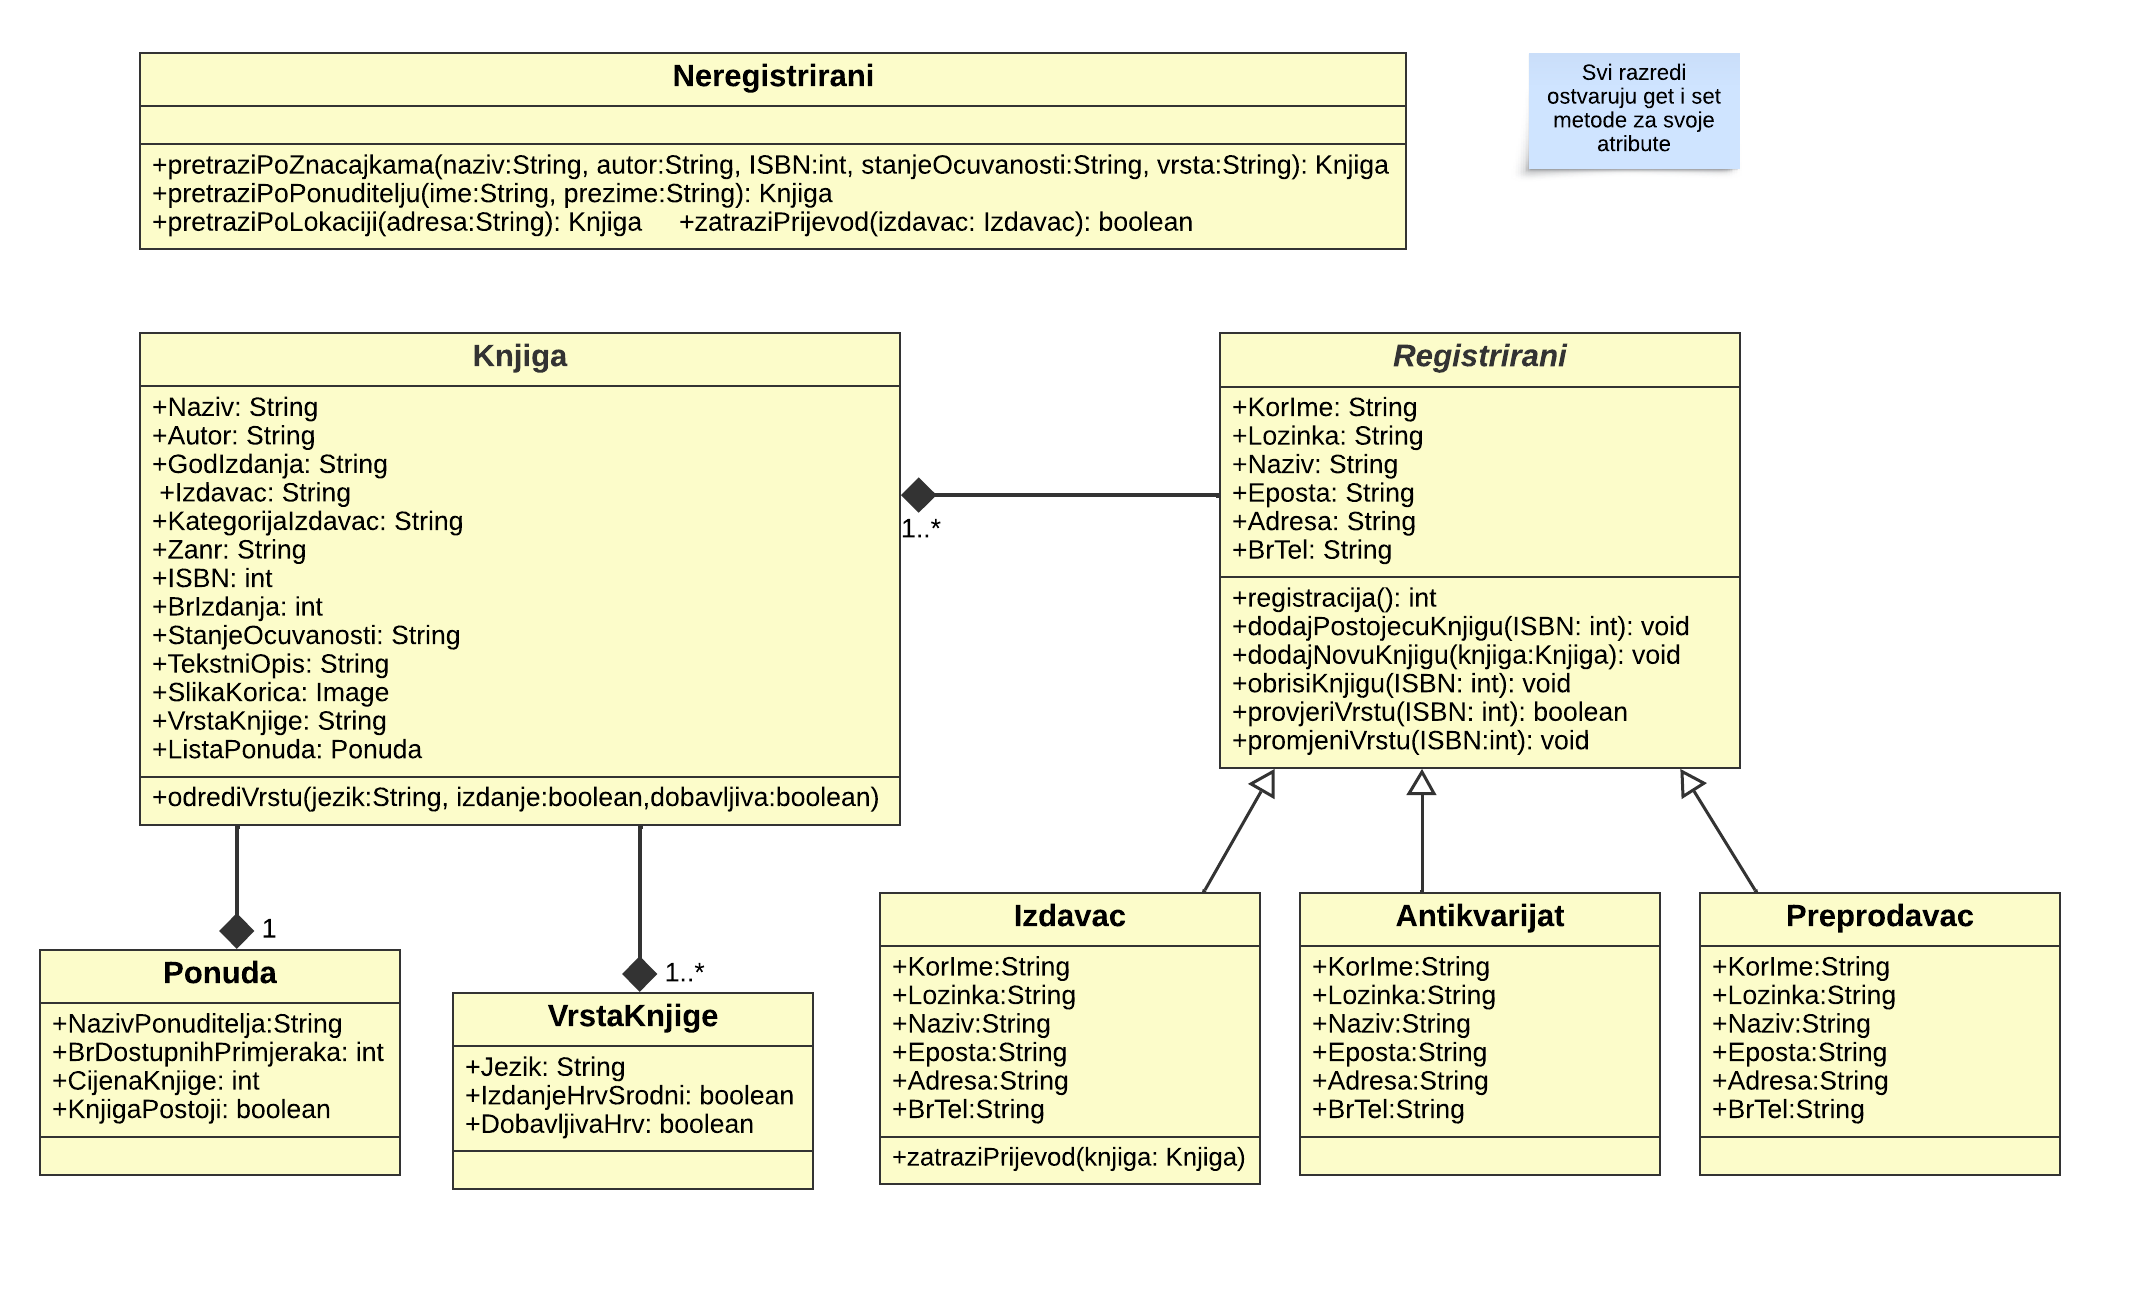
\includegraphics[width = \textwidth]{slike/dijagramKlasa.PNG}
				\caption{Dijagram razreda}
				\label{fig:enter-label}
			\end{figure}
			
			
			\textbf{\textit{dio 2. revizije}}\\			
			
			\textit{Prilikom druge predaje projekta dijagram razreda i opisi moraju odgovarati stvarnom stanju implementacije}
			
			
			
			\eject
		
		\section{Dijagram stanja}
			
			
			\textbf{\textit{dio 2. revizije}}\\
			
			\textit{Potrebno je priložiti dijagram stanja i opisati ga. Dovoljan je jedan dijagram stanja koji prikazuje \textbf{značajan dio funkcionalnosti} sustava. Na primjer, stanja korisničkog sučelja i tijek korištenja neke ključne funkcionalnosti jesu značajan dio sustava, a registracija i prijava nisu. }
			
			
			\eject 
		
		\section{Dijagram aktivnosti}
			
			\textbf{\textit{dio 2. revizije}}\\
			
			 \textit{Potrebno je priložiti dijagram aktivnosti s pripadajućim opisom. Dijagram aktivnosti treba prikazivati značajan dio sustava.}
			
			\eject
		\section{Dijagram komponenti}
		
			\textbf{\textit{dio 2. revizije}}\\
		
			 \textit{Potrebno je priložiti dijagram komponenti s pripadajućim opisom. Dijagram komponenti treba prikazivati strukturu cijele aplikacije.}